\documentclass{article}
\usepackage{ctex}
\usepackage{amssymb, amsmath}
\usepackage[margin=1in]{geometry}
\usepackage{graphicx}
\usepackage{enumitem}
\setlist[enumerate]{topsep=.5ex, partopsep=0ex, parsep=.5ex, itemsep=0ex}
\usepackage{mathptmx}
\begin{document}
蝶式价差(butterfly spread)的名字相当奇异,它实际上是一个中性价差,是一手牛市价差同一手熊市价差的组合。\textit{这个价差适用于对市场持中立观点的策略家,这个策略家认为标的股票在期权到期之前净上涨或净下跌都不会太大}。这个策略一般只需要小额的投资,风险也有限。虽然它们的盈利也有限,但它们的潜在盈利要大于潜在风险。由于这个原因,蝶式价差是一个有活力的策略。不过,就手续费而言,它相当昂贵。这里,我们只介绍使用看涨期权的蝶式价差。当然,这个价差既可以使用看涨期权同看跌期权的结合,也可以只用看跌期权来构建。

一个蝶式价差中有 3 个行权价。如果只使用看涨期权,蝶式价差包括买入 1 手行权价最低的看涨期权,卖出 2 手中间行权价的看涨期权,和买入 1 手行权价最高的看涨期权。同一般情况一样,最大数量的盈利是在卖出的看涨期权的行权价上实现的。对大多数类型的价差,记住这个事实很有用,因为它可以帮助你迅速计算出这个价差的潜在盈利。

\begin{figure}[h]
    \centering
    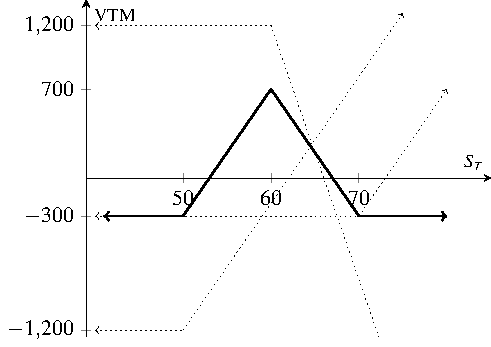
\includegraphics[width=0.7\textwidth]{../IMG/pngbutterflyspreads.pdf}
    \caption{条件:$K_1=50, K_2=60, K_3=70, c_1=12, c_2=6, c_3=3, m=100$}
    \label{fig:call_spread}
\end{figure}

如果期权是同一月份到期,而且行权价之间差距相等,那么,就可以使用下面的公式迅速地计算出这手蝶式价差的重要细节:
\begin{equation}
    \begin{aligned}
    \text{净投资}&=\text{价差的净支出}\\
    \text{最大盈利}&=\text{行权价之间的差距}-\text{净支出}\\
    \text{下行盈亏平衡点}&=\text{最低行权价}+\text{净支出}\\
    \text{上行盈亏平衡点}&=\text{最高行权价}-\text{净支出}\\
    \end{aligned}
\end{equation}

\section{选择价差}
理想情况下,投资者会希望能用尽量小的支出来建立一手蝶式价差,从而将他的风险限制在最小的程度,尽管最小风险的金额仍然等于其在这个价差中 100\% 的投资。

最小支出蝶式价差是那些股票价格与中间行权价有某些距离的价差。要说明这一点,请注意,如果股票高出中间行权价一定距离而且所有的期权都处于持平状态的话,净支出就会是零。因为存在提前指派的风险,没有人会想要用持平的期权建立一手蝶式价差。但如果试图对标的股票的期权进行选择,从而获得一个较小的支出,那这样做会有一定的好处。例如,如果股票接近于较高的行权价,支出一般而言会比较小,但投资者就必须在某种程度上对标的股票看空,这样才能在最大限度上实现他的盈利。也就是说,为了实现最大盈利,股票的价格就必须从较高的行权价下跌到中间的行权价。相似的情况也存在于当股票一开始接近较低的行权价的时候。在这种情况里,投资者也可以用少量的支出建立这个价差,但是,此时如果他想要实现他的最大盈利,就必须对标的股票持某种看多的态度。
\end{document}